\documentclass[11pt,a4paper,headsepline,hidelinks]{scrreprt} % KOMA-Script
\usepackage[italian]{babel}
\usepackage[utf8]{inputenc}
\usepackage[T1]{fontenc}
\usepackage{graphicx}
\usepackage{amsfonts}
\usepackage{amsmath}
\usepackage{hyperref}
\pagestyle{headings}
\renewcommand{\arraystretch}{1.5}

\begin{document}
  \title{Relazione di stage - Bozza}
	\subject{Analisi e progettazione di un'interfaccia grafica per la consultazione dei contenuti informativi in una piattaforma web tematica}
  \author{Nicola Moretto (matr. 578258)}
  \date{\today}

  \maketitle

	\tableofcontents

	\listoffigures
	\begingroup
	\let\clearpage\relax
	\listoftables
	\endgroup
	
	\begin{abstract}
	\chapter*{Sommario}
	L'attività di stage si è svolta presso l'azienda \textit{Sintesi Sas}, che opera nel settore ICT (\textit{Information and Comunication Technology}) realizzando software ERP e piattaforme Web per aziende, in particolare attive nel settore turistico, e fornendo servizi di consulenza e di formazione di imprenditori nell'ambito del marketing strategico, operativo e del controllo di gestione.
	
	Il prodotto di punta dell'azienda - \textit{Planet Hotel} - costituisce un sistema software per la gestione alberghiera tra i più flessibili, ampi e completi presenti nel panorama italiano, in grado di coprire la maggior parte delle necessità aziendali: oltre alla gestione delle prenotazioni e dei conti, esso offre un insieme di moduli integrati per supportare il controllo di gestione e degli interventi di marketing.

	Si tratta di una realtà imprenditoriale a clientela nazionale con sede unica a Mestre (VE), la cui direzione e amministrazione è affidata al solo fondatore, che ha assunto il ruolo di tutor esterno e referente aziendale per l'intera durata dello stage.

	Le attività svolte si inseriscono nell'ambito di un progetto esterno rispetto al business dell'azienda. finalizzato alla realizzazione di una piattaforma web tematica per la condivisione di informazioni e la vendita diretta di prodotti alla clientela, e affidato ad un team costituito da differenti figure professionali (sociologi, informatici, ingegneri, \ldots).
	
	\section*{Contenuti}
	Il presente documento costituisce una relazione dettagliata in merito all'attività di stage svolta dallo studente Nicola Moretto presso l'azienda \textit{Sintesi Srl}. I contenuti sono organizzati nei seguenti capitoli:
	\begin{description}
		\item[\nameref{ch:tesi:progetto}] \hfill \\
		Il primo capitolo illustra le strategie dell'azienda e gli obiettivi, i requisiti e i vincoli del progetto in cui si inseriscono le attività di stage.
		\item[\nameref{ch:tesi:stage}] \hfill \\ 
		Il secondo capitolo illustra gli obiettivi, i requisiti e l'organizzazione (piano e norme di lavoro) delle attività di stage. A seguire vengono presentate le scelte più rilevanti effettuate e i risultati conseguiti.
		\item[\nameref{ch:tesi:valutazioni}] \hfill \\
		Il terzo capitolo presenta un'analisi critica a posteriori dell'attività di stage: raggiungimento degli obiettivi prefissati, competenze professionali acquisite, \ldots.
	\end{description}

	\section*{Convenzioni tipografiche}
	Al fine di agevolare la consultazione del documento sono state adottate alcune convenzioni tipografiche illustrate di seguito.

	\paragraph{Glossario} Gli acronimi, le abbreviazioni, i nomi propri e i termini specialistici contenuti nel presente documento sono illustrati nel \textit{\nameref{ch:tesi:appendice:glossario}}, consultabile in appendice, al fine di agevolare la lettura e la comprensione degli argomenti trattati. La prima occorrenza di ciascun termine o espressione presente nel glossario appare \underline{sottolineata}.

	\paragraph{Terminologia} La prima occorrenza di termini propri o di provenienza straniera divenuti di uso corrente nella lingua italiana sono evidenziati in \textit{corsivo}, mentre le parole o espressioni che assumono particolare significato nel presente contesto sono riportate in \textsc{maiuscoletto}.

	\paragraph{Codice e formule} I nomi di tabelle, classi, package, \ldots\ impiegano uno stile di carattere \textsf{sans serif}, mentre i frammenti di codice o formule impiegano un carattere a \texttt{spaziatura fissa}.
	
	\end{abstract}

	%=========
	% CONTENTS
	%=========
	%\chapter{Introduzione}
\label{ch:tesi:intro}

\section{Contenuti}
Il presente documento costituisce una relazione dettagliata in merito all'attività di stage svolta dallo studente Nicola Moretto presso l'azienda \textit{Sintesi Srl}. I contenuti sono organizzati nei seguenti capitoli:
\begin{description}
  \item[\nameref{ch:tesi:intro}] \hfill \\
  Il primo capitolo illustra brevemente la struttura del documento e le convenzioni tipografiche utilizzate.
  \item[\nameref{ch:tesi:progetto}] \hfill \\
  Il secondo capitolo illustra le strategie dell'azienda e gli obiettivi, i requisiti e i vincoli del progetto in cui si inseriscono le attività di stage.
  \item[\nameref{ch:tesi:stage}] \hfill \\ 
	Il terzo capitolo illustra gli obiettivi, i requisiti e l'organizzazione (piano e norme di lavoro) delle attività di stage. A seguire vengono presentate le scelte più rilevanti effettuate e i risultati conseguiti.
  \item[\nameref{ch:tesi:valutazioni}] \hfill \\
	Il quarto capitolo presenta un'analisi critica a posteriori dell'attività di stage: raggiungimento degli obiettivi prefissati, competenze professionali acquisite, \ldots.
\end{description}

\section{Convenzioni tipografiche}
Al fine di agevolare la consultazione del documento, sono state adottate alcune convenzioni tipografiche illustrate di seguito.

\paragraph{Glossario} Gli acronimi, le abbreviazioni, i nomi propri e i termini specialistici contenuti nel presente documento sono illustrati nel \textit{\nameref{ch:appendice:glossario}}, consultabile in appendice, al fine di agevolare la lettura e la comprensione degli argomenti trattati.	La prima occorrenza di ciascun termine o espressione presente nel glossario è riconoscibile per la \underline{sottolineatura}.

\paragraph{Terminologia} La prima occorrenza di termini propri o di provenienza straniera divenuti di uso corrente nella lingua italiana sono evidenziati in \textit{corsivo}, mentre per le parole o espressioni che assumono particolare significato nel presente contesto si ricorre al \textsc{maiuscoletto}.

\paragraph{Codice e formule} I nomi di tabelle, classi, package, \ldots sono riportati con un carattere di tipo \textsf{sans serif}, mentre i frammenti di codice o formule sono riconoscibili per l'impiego di un carattere a \texttt{spaziatura fissa}.

	\chapter{Progetto}
\label{ch:tesi:progetto}

\section{Genesi}
\label{sec:tesi:progetto:genesi}
L'idea della piattaforma \textit{Social (Life) Shuttle} nasce nel 2010 da un progetto concepito per dar vita ad una comunità virtuale destinata agli artisti sconosciuti e accessibile in mobilità mediante un'applicazione dedicata, \textit{ArtYR}.

Nello stesso periodo una consulenza nell'ambito dei sistemi informativi territoriali ad un'azienda di Bolzano conduce allo sviluppo di un'innovativa piattaforma software: un sistema informativo territoriale in cui l'erogazione di informazioni turistiche è integrata con la vendita di servizi turistici.

Il progetto evolve - grazie alla partecipazione di Comuni, Province e Regioni - in una rete tematica di agenzie di viaggio con un'identità comune e finalizzata alla fusione dei sistemi informativi distrettuali e di vendita.

L'architettura di \textit{Social (Life) Shuttle} trae profonda ispirazione, integrando tre componenti differenti:
\begin{description}
	\item[Business] \hfill \\
	Vendita diretta di prodotti alla clientela.
	\item[Sociale] \hfill \\
	Creazione e sviluppo delle relazioni sociali attraverso la condivisione di informazioni e conoscenza.
	\item[Territorio] \hfill \\
	Sistema di erogazione di informazioni turistiche e territoriali.
\end{description}

\section{Reti sociali}
\label{sec:tesi:progetto:reti-sociali}
Il modello sociologico di \underline{rete sociale} non ha attualmente riscontro presso le piattaforme web di condivisione dei contenuti (\textit{blog}, \textit{forum}, \ldots) o i \textit{social network} (Facebook, Twitter, \ldots), che si limitano a considerarne e concretizzarne singoli aspetti.

Nelle moderne reti sociali è infatti assente l'incentivo alla condivisione e distribuzione della conoscenza, fattore cruciale per l'aggregazione fisica dei membri delle comunità, da intendersi a sua volta come aggregazioni formatesi intorno ed attraverso la manifestazione di interesse nei confronti di uno specifico tema di dialogo o discussione che attraversa la sfera individuale, intima e personale dei suoi membri.

Il progetto \textit{Social (Life) Shuttle} rappresenta una nuova generazione di piattaforma di socializzazione, in cui il web diventa solamente un canale di condivisione e un serbatoio della conoscenza generata dalla dialettica tra persone e dove vengono integrati i canoni classici di \textit{blog}, \textit{forum}, \textit{social network} e \textit{media} .

Una relazione sociale nata e costruita su un interesse comune stravolge l'attuale paradigma delle reti sociali virtuali, in cui il legame nasce a prescindere dalla presenza di interessi comuni o informazioni da condividere, e favorisce l'incontro tra persone aventi esperienze simili frutto di tali interessi condivisi. Ove l'esperienza riguardi anche beni o prodotti, la componente business intende offrire ai membri la possibilità di interagire con i produttori, anch'essi attori della comunità.

L'architettura di \textit{Social (Life) Shuttle} consente di declinare la piattaforma in innumerevoli varianti, applicabili ai temi più svariati: al momento sono in fase di sperimentazione per il mondo del vino, il cibo biologico, l'arte commercializzabile e l'attività di ricerca e progettazione collaborativa. 

\section{Architettura}
\label{sec:tesi:progetto:architettura}
Tale piattaforma presenta numerose aspetti che la differenziano dalla concorrenza attuale:
\begin{itemize}
	\item profonda integrazione degli aspetti \textit{social} e \textit{business};
	\item nessuna distinzione tra creatori e fruitori dei contenuti (ciascun membro può condividere le proprie esperienze, segnalare eventi, pubblicare articoli critici, \ldots);
	\item l'autorevolezza di ciascun membro della comunità si rafforza o si indebolisce a seconda della qualità dei contenuti pubblicati, dei giudizi degli altri membri e di altri criteri di valutazione;
	\item lo sfruttamento di tecnologie e dispositivi mobili per favorire la crescita di relazioni al di fuori dell'ambito virtuale della piattaforma (partecipazione ad eventi, raccolta e condivisione di informazioni geolocalizzate, \ldots).
\end{itemize}

\begin{figure}[ht]
	\begin{center}
		
\includegraphics{placeholder.png}
		\label{fig:tesi:progetto:gerarchia-utenti}
		\caption{Gerarchia degli utenti nelle piattaforme web tradizionali}
	\end{center}
\end{figure}

% definizione di rete sociale: Granovetter.
Per quanto concerne le attività di stage, due aspetti della piattaforma assumono particolare rilevanza: i contenuti informativi e i relativi criteri di classificazione.

\subsection{Contenuti informativi}
\label{sec:tesi:progetto:contenuti}
I contenuti informativi rappresentano lo strumento essenziale per la condivisione delle esperienze e della conoscenza intorno al tema specifico della piattaforma.

Per individuare le classi di contenuti adatte a esprimere in una forma strutturata le informazioni si è tratta ispirazione dalle forme espressive e comunicative tipiche della dialettica quotidiana, poiché risultano immediatamente e intuitivamente comprensibili agli utenti, a prescindere dal loro livello di esperienza.

In particolare, si distinguono la natura della comunicazione, connessa allo scopo e al tono con cui ci esprimiamo, e il formato delle informazioni, che dipendono strettamente dai sensi e dai canali di comunicazione a disposizione per scambiare informazioni con l'interlocutore, sia esso un individuo singolo o un gruppo.

\paragraph{Classi}
I tipi di contenuto pubblicabili nella piattaforma dovrebbero essere in numero adeguato a coprire il maggior numero possibile di esigenze comunicative pur rimanendo facilmente e intuitivamente distinguibili, ossia l'utente non dovrebbe nutrire dubbi circa il più adatto a formalizzare di volta in volta l'informazione che desidera condividere.
\begin{description}
\item[Domanda] \hfill \\
La domanda classica rende particolarmente esplicito lo scopo della comunicazione, ossia la richiesta di informazioni di varia natura agli altri utenti della piattaforma. Si distingue in pubblica o privata, a seconda che l'utente desideri rivolgerla ad un particolare sottoinsieme di utenti. 
\item[Risposta] \hfill \\
Duale della domanda, la risposta è anch'essa in forma pubblica o privata per consentire all'utente di renderla accessibile e consultabile solo a certi utenti, spesso l'autore della domanda a cui risponde.
\item[Pensierino] \hfill \\
Il pensierino rappresenta una forma di comunicazione adatta ad esprimere un contenuto di lunghezza breve e con contenuti superficiali (considerazioni, stati d'animo, freddure, \ldots).
\item[Evento] \hfill \\
L'evento identifica e aiuta a promuovere qualsiasi iniziativa che rientri nell'ambito tematico della piattaforma e cui possano prender parte altre persone (incontro pubblico, concerto, fiera, \ldots).
\item[Discorso] \hfill \\
Il discorso identifica un contenuto articolato, sia nella forma sia nei contenuti, destinato alla condivisione di informazioni dettagliate e approfondite.
\item[Recensione] \hfill \\
La recensione esprime un giudizio critico nei confronti di un prodotto specifico. 
\item[Comunicazione privata] \hfill \\
La comunicazione privata è l'unica forma di contatto diretto e riservato tra due utenti.
\end{description}

\paragraph{Elementi}
Ciascun tipo di contenuto esprime un intento comunicativo ben preciso, ma non è vincolato ad una struttura e ad un formato predefiniti: la classe, che esprime l'intento della comunicazione, si colloca in un piano distinto rispetto al formato, ossia la struttura e le caratteristiche specifiche del contenuto informativo condiviso.

Ove la dialettica quotidiana dispone infatti di cinque sensi e può esprimersi in forma non solo verbale, nel web gli utenti sperimentano differenti forme di comunicazione: contenuti testuali e grafici, flussi audio e video, documenti elettronici, messaggistica istantanea, \ldots\ .

I contenuti informativi non presentano dunque una struttura fissa a seconda della classe ma possono essere liberamente redatti a partire da una serie di elementi predefiniti, frutto di una ricerca tra le principali e più diffuse piattaforme web disponibili (\textit{blog}, \textit{forum}, \textit{social network}, \textit{chat}, \ldots) e di una successiva analisi e rielaborazione dei risultati ottenuti:
\begin{description}
\item[Audio] \hfill \\
Contenuto audio statico o in tempo reale (\textit{live streaming}, \ldots).
\item[Immagini] \hfill \\
Contenuto grafico statico.
\item[Video] \hfill \\
Contenuto video statico o in tempo reale (\textit{live streaming}, \ldots).
\item[Sondaggio] \hfill \\
Domanda a risposta multipla.
\item[Documento] \hfill \\
File di testo o binario caricato nella piattaforma.
\item[Stringa] \hfill \\
Contenuto testuale avanzato (intestazioni, formattazione dei caratteri, collegamenti ipertestuali, \ldots).
\item[Citazione] \hfill \\
Citazioni o riferimenti ad altri elementi di un contenuto, ad un contenuto informativo o a prodotti presenti nella piattaforma. 
\end{description}

\begin{figure}[ht]
	\begin{center}
		
\includegraphics{placeholder.png}
		\label{fig:tesi:progetto:contenuti-informativi}
		\caption{Struttura di un contenuto informativo}
	\end{center}
\end{figure}

La struttura modulare dei contenuti informativi consente di riusare, riferire o citare gli elementi costituenti e di catalogarli con maggior facilità e precisione, riuscendo a classificare ciascun frammento di informazione presente al loro interno.

\paragraph{Proprietà}
I contenuti informativi - a prescindere dalla classe e dalla struttura - presentano un insieme di proprietà comuni, alcune delle quali assumono particolare rilevanza per l'attività di stage, rappresentando utili criteri addizionali per filtrare i contenuti informativi durante una ricerca: si tratta di \textsc{autore}, \textsc{data di pubblicazione} e \textsc{tipo} del contenuto.

\paragraph{Relazioni}
Ove tradizionalmente ci si affida ai commenti per consentire agli utenti di esprimere un'opinione rispetto alle informazioni riportate o alle posizioni espresse in un contenuto, in \textit{Social (Life) Shuttle} si permette di rispondere ad un contenuto pubblicato nella piattaforma direttamente con altri contenuti, in numero arbitrario.

La relazione di dipendenza tra i contenuti prescinde dalla classe specifica, non ponendo vincoli di alcun genere circa la classe ed il formato della risposta ad un contenuto informativo.

Ciò consente maggiore libertà all'utente nello scegliere la forma espressiva più adeguata per condividere il proprio messaggio, ne facilita la catalogazione e allo stesso tempo rispecchia il principio di uguaglianza tra gli utenti espresso in precedenza ed elemento cardine della piattaforma.

Nel corso del tempo a partire da ciascun contenuto informativo possono così svilupparsi e ramificarsi diverse \textsc{discussioni}, senza limiti di ampiezza o profondità.

\subsection{Sistema di classificazione}
\label{sec:tesi:progetto:classificazione}
Il sistema di classificazione consiste in un insieme di criteri che associano a ciascun contenuto alcuni metadati, in grado di fornire agli utenti della piattaforma informazioni utili a contestualizzarlo, ad interpretarlo e a valutarne l'interesse soggettivo:
\begin{description}
 	\item[Argomento] \hfill \\
 	L'argomento di un contenuto rappresenta la branca del sapere - agnostica rispetto al tema specifico della piattaforma - cui appartiene. 
 	\item[Emozioni] \hfill \\
 	Le emozioni indicano lo stato d'animo con cui un contenuto sia stato pubblicato dall'autore.
 	\item[Giudizi] \hfill \\
 	I giudizi forniscono una valutazione qualitativa sul contenuto e sono espressi dagli utenti.
 	\item[Intenzioni] \hfill \\
 	Le intenzioni indicano lo spirito con cui l'autore redige il contenuto (opinione, critica, \ldots).
 	\item[Interessi] \hfill \\
 	Gli interessi rappresentano temi specifici della piattaforma nei confronti dei quali ciascun utente registrato dichiara di nutrire passione.
\end{description}

Queste meta-informazioni assumono particolare rilevanza nel processo di ricerca di informazioni all'interno della piattaforma, poiché consentono di escludere o meno determinati contenuti dai risultati.

Tra quelli evidenziati, tuttavia, spicca l'assenza di un criterio in grado di catalogare ordinatamente le informazioni presenti nei contenuti per facilitarne la ricerca, il reperimento e la consultazione: il primo obiettivo dell'attività di stage consiste nell'individuare un meccanismo efficiente per rendere più agevole la consultazione della conoscenza custodita nella piattaforma, fornendo un livello di astrazione rispetto alla semplice enumerazione dei contenuti.

\section{Requisiti e vincoli}
\label{sec:tesi:progetto:requisiti}
Durante gli incontri preliminari all'attività di stage sono stati fissati gli obiettivi, i requisiti ed i vincoli concernenti le attività previste ed i prodotti attesi. 

\subsection{Criterio di classificazione}
\label{sec:tesi:progetto:requisiti:criterio-classificazione}
La progettazione del criterio di classificazione deve tenere conto di alcuni vincoli e requisiti riguardanti l'integrazione con il sistema di classificazione e l'architettura della piattaforma:

\begin{description}
	\item[Indipendenza dai criteri esistenti] \hfill \\
	Il criterio deve minimizzare il grado di accoppiamento per risultare facilmente mantenibile e aggiornabile senza intaccare lo stato, l'integrità e le funzionalità dei rimanenti e deve tenere conto di possibili evoluzioni della piattaforma, che comportino l'aggiornamento o la rimozione dei criteri esistenti o l'aggiunta di nuovi.
	\item[Indipendenza dalle classi di contenuti] \hfill \\
	Il criterio non deve distinguere tra contenuti di classi diverse, ma deve considerare esclusivamente le proprietà e le relazioni definibili a livello del contenuto generico.
	\item[Indipendenza dalle componenti del sistema] \hfill \\
	Il criterio deve minimizzare le dipendenze e l'accoppiamento con le altre componenti del sistema, che possono essere soggette ad aggiornamenti sostanziali (in particolare per quelle di terze parti) o interventi di manutenzione evolutiva.
	\item[Modularità] \hfill \\
	Il criterio dev'essere progettato in modo tale da potersi avvantaggiare in futuro di soluzioni tecniche o tecnologiche in grado di automatizzare (in parte o del tutto) le operazioni di classificazione dei contenuti (motori di ricerca semantica, \ldots);
\end{description}

Le potenziali criticità tecniche, legate all'implementazione del criterio di classificazione, devono essere raccolte e condivise con il team di progetto, che provvederà a valutarle, a fornire eventuali indicazioni e ad individuare le soluzioni ritenute appropriate e compatibili con l'architettura e le specifiche della piattaforma.

\subsection{Interfaccia grafica}
\label{sec:tesi:progetto:requisiti:interfaccia-grafica}
L'interfaccia grafica per la consultazione dei risultati di una ricerca sui contenuti informativi deve soddisfare alcuni requisiti essenziali.

\paragraph{Requisiti funzionali}
\begin{itemize}
	\item Deve consentire all'utente di inserire dei termini di ricerca e selezionare un ambito;
	\item deve potersi interfacciare a componenti terze per ottenere i risultati di ricerca;
	\item deve mostrare i contenuti con forme geometriche elementari, che permettano di distinguerne intuitivamente la classe di appartenenza;
	\item deve permettere la consultazione della discussione associata ad un contenuto, evidenziando il flusso informativo (sequenze di risposte ad un contenuto):
	\item dovrebbe gestire dei filtri basati sugli interessi ed il livello di esperienza di un utente registrato.
\end{itemize}

\paragraph{Requisiti di qualità}
\begin{itemize}
	\item dev'essere in grado di visualizzare ordinatamente un numero elevato di risultati di ricerca;
	\item dev'essere utilizzabile agevolmente da utenti con differenti livelli di esperienza;
	\item dev'essere adeguatamente fruibile su dispositivi mobili.
\end{itemize}

	\chapter{Stage}
\label{ch:tesi:stage}

\section{Piano di stage}
\label{sec:tesi:stage:piano}

\subsection{Obiettivi e requisiti}
\label{sec:tesi:stage:piano:obiettivi}
L'attività di stage si colloca nell'ambito del progetto presentato nel capitolo \ref{ch:tesi:progetto} e persegue due obiettivi distinti ma correlati, focalizzandosi sulla componente \textit{social} della piattaforma.

\paragraph{Criterio di classificazione}
Il primo obiettivo consiste nell'estendere l'attuale sistema di classificazione (v. sezione \ref{sec:tesi:progetto:classificazione}), integrandovi un criterio aggiuntivo per la catalogazione dei contenuti pubblicati dagli utenti e la costruzione di un'enciclopedia della conoscenza, al fine di rendere il reperimento e la consultazione delle informazioni desiderate il più efficiente ed agevole possibile.

L'ideazione e concezione del suddetto criterio deve tener conto della natura tematica della piattaforma, conciliando due esigenze distinte:
\begin{itemize}
\item dev'essere sufficientemente astratto e flessibile per adattarsi alla molteplicità di varianti tematiche in cui la piattaforma stessa può essere declinata;
\item deve cercare di avvantaggiarsi delle peculiarità di una piattaforma tematica, ad esempio la maggior correlazione degli argomenti trattati.
\end{itemize}

La soluzione individuata deve inoltre prescindere da assunzioni legate alla tecnologia utilizzata.

Alla luce di possibili evoluzioni nello sviluppo della piattaforma, si desidera infine che la classificazione di un contenuto informativo (assegnazione di metadati, individuazione di correlazioni, \ldots) possa essere - in futuro - demandata a componenti software integrate nella piattaforma.

\paragraph{Interfaccia grafica}
Il secondo obiettivo consiste nel progettare un'interfaccia grafica per la consultazione dei contenuti informativi, che sfrutti il criterio di classificazione aggiuntivo per facilitare la ricerca ed il reperimento delle informazioni di interesse per l'utente all'interno del patrimonio enciclopedico della piattaforma.

La sfida principale consiste nel progettare un'interfaccia in grado di visualizzare in maniera chiara e ordinata un numero arbitrario di contenuti, a prescindere dalla classe del dispositivo impiegato (\textit{smartphone}, \textit{tablet}, \textit{notebook}, \ldots).

Il primo passo consiste nell'individuare le informazioni essenziali per una rapida e precisa identificazione dei contenuti (titolo, autore, data di pubblicazione, \ldots) e nel valutare la notazione (grafica o testuale) più adatta per esprimerle, al fine di renderle accessibili al maggior numero possibile di utenti; le informazioni aggiuntive devono risultare comunque accessibili, ma solo su esplicita richiesta dell'utente.

In questo frangente si inseriscono alcune analisi e valutazioni di carattere sociologico, svolte da altri membri del team di progetto, per individuare le soluzioni più idonee a comunicare tali informazioni in modo da renderne la comprensione chiara e intuitiva a qualsiasi utente.

Il secondo passo richiede di definire le specifiche per un'interfaccia facilmente navigabile, che sia in grado di mostrare in modo ordinato e intuitivo i contenuti e le reciproche relazioni. Occorre individuare opportuni criteri di raggruppamento, ordinamento e collocazione dei contenuti visualizzati per favorirne la consultazione, evitando un sovraccarico cognitivo e garantendo un livello adeguato di leggibilità.

Con il terzo ed ultimo passo si mira ad aggiungere la possibilità per l'utente di filtrare i contenuti visualizzati in accordo a proprietà (argomento, autore, data di pubblicazione, tipo) o metadati associati (emozioni, giudizi, intenzioni, \ldots).

Per gli utenti autenticati si desidera offrire un livello aggiuntivo di personalizzazione, che consenta di filtrare automaticamente i contenuti secondo le preferenze associate al profilo (interessi, livello di esperienza).

Per individuare i requisiti essenziali si prendono in considerazione alcuni casi d'uso:
\begin{enumerate}
\item l'utente naviga liberamente tra i contenuti (più recenti, più letti, più discussi, \ldots);
\item l'utente consulta la discussione generata da un singolo contenuto;
\item l'utente cerca le informazioni riguardanti un certo tema;
\item l'utente esplora gli argomenti trattati e le reciproche relazioni.
\end{enumerate}

\subsection{Pianificazione}
L'attività di stage viene suddivisa in due fasi distinte per semplificarne la pianificazione:
\begin{enumerate}
\item l'estensione del sistema di classificazione;
\item l'analisi e la progettazione dell'interfaccia grafica.
\end{enumerate}

Per ciascuna fase sono fissati gli obiettivi generali, sono individuate e organizzate su base settimanale le attività da svolgere, cercando di garantire un carico di lavoro equilibrato, e sono indicati i prodotti attesi.

La durata complessiva dello stage si attesta su 8 settimane a tempo pieno, corrispondenti a 320 ore di lavoro.

\begin{table}[ht]
\centering
\begin{tabular}{|p{11cm}|p{1cm}|}
\hline
\textsc{Attività} & \textsc{Ore} \\ \hline
\multicolumn{2}{|c|}{\textit{Fase 1: estensione del sistema di classificazione}} \\ \hline 
Analisi delle specifiche del sistema di classificazione & 40 \\ \hline
Analisi comparativa dei principali sistemi di classificazione della conoscenza & 40 \\ \hline
Progettazione del sistema di classificazione & 40 \\ \hline
Implementazione del sistema di classificazione nel modello relazionale & 40 \\ \hline
\multicolumn{2}{|c|}{\textit{Fase 2: analisi e progettazione dell'interfaccia grafica}} \\ \hline 
Analisi dei requisiti dell'interfaccia grafica & 40 \\ \hline
Progettazione dell'interfaccia grafica: visualizzazione dei contenuti & 40 \\ \hline
Progettazione dell'interfaccia grafica: filtraggio dei contenuti & 40 \\ \hline
Progettazione dell'interfaccia grafica: navigazione dei contenuti & 40 \\ \hline
\end{tabular}
\caption{Pianificazione settimanale delle attività}
\label{tab:tesi:stage:pianificazione}
\end{table}

\begin{figure}[ht]
	\begin{center}
		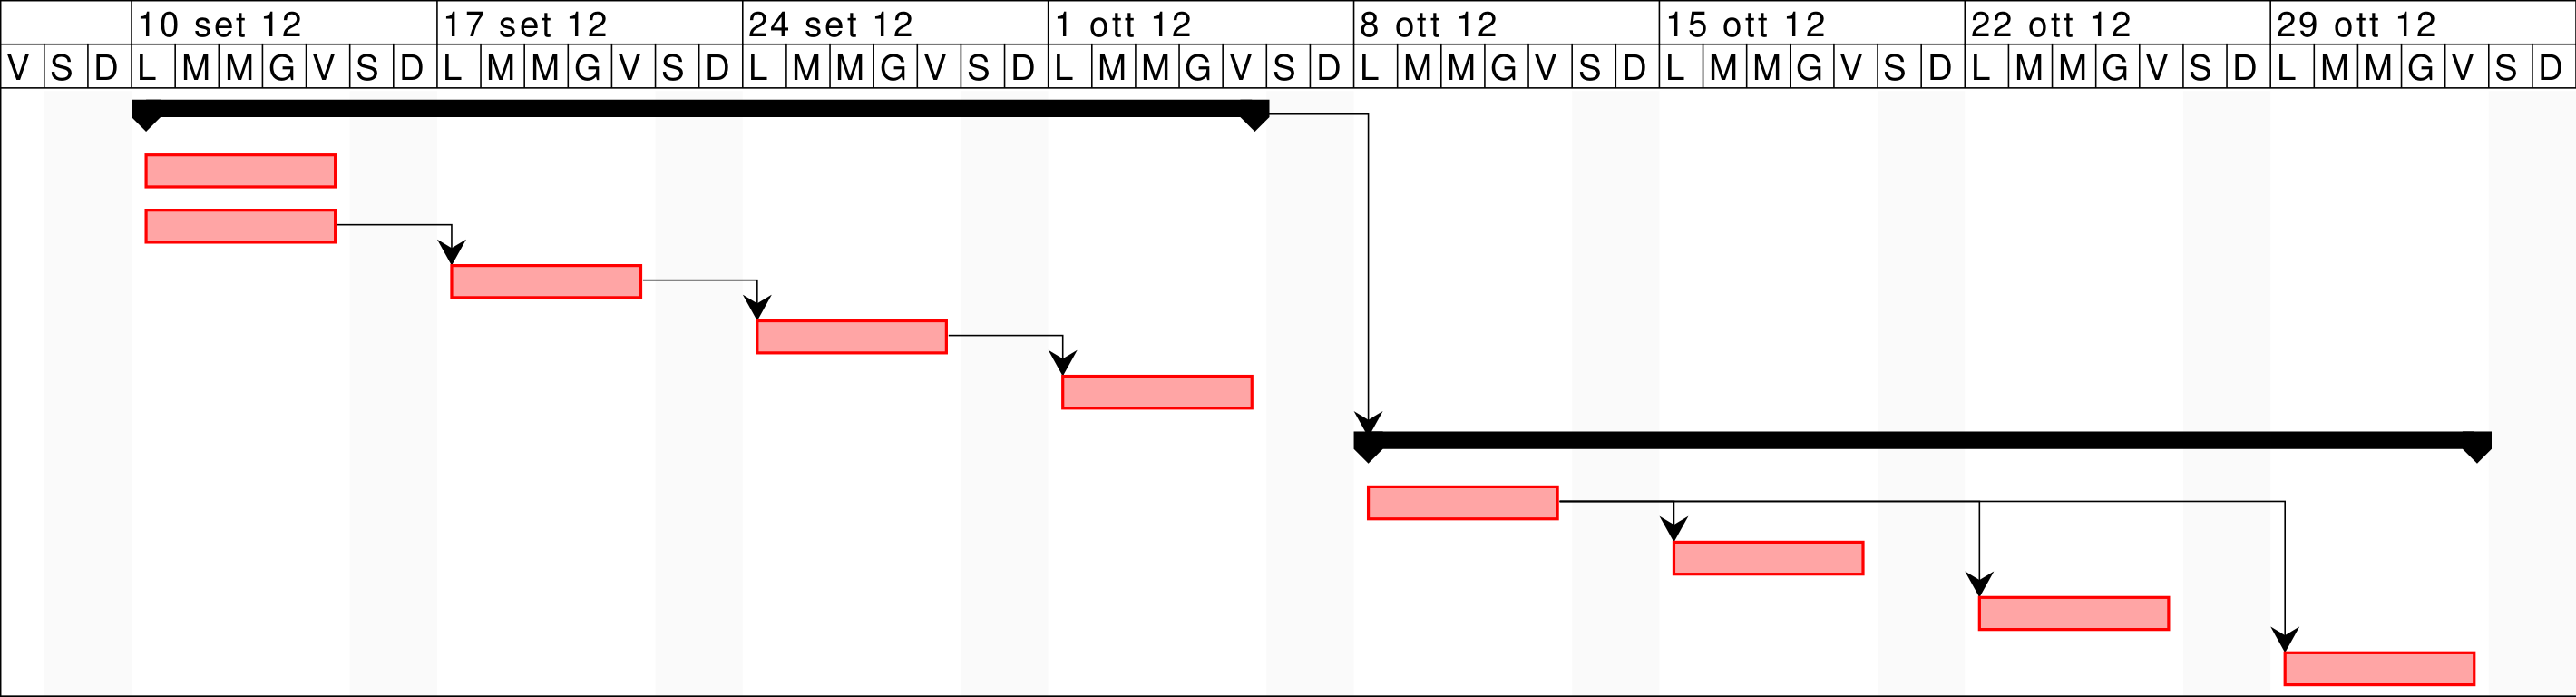
\includegraphics[width=13cm]{img/gantt.png}
		\label{fig:tesi:stage:gantt}
		\caption{Diagramma di Gantt}
	\end{center}
\end{figure}

\section{Norme di stage}
Nel corso dello stage sono stati impiegati diversi strumenti per gestire le attività di progetto e produrre la documentazione prevista.

\begin{table}[ht]
\centering
\begin{tabular}{|l|l|}
\hline
\textsc{Controllo di versione} & \underline{Mercurial} 2.0.2 \\ \hline
\textsc{Editor \LaTeX} & \underline{LaTeXila} 2.4.0 - \underline{gedit} 3.4.0\\ \hline
\textsc{Editor UML} & \underline{UMLet} 11.5.1 \\ \hline
\textsc{Foglio elettronico} & \underline{LibreOffice Calc} 3.6 \\ \hline
\textsc{Gestione database} & \underline{MySQL Workbench} 5.2.42 \\ \hline
\textsc{Mockup} & \underline{Pencil} 2.0.2 \\	\hline
\textsc{Pianificazione} & \underline{ProjectLibre} 1.5.1 \\ \hline
\textsc{Repository} & \underline{Bitbucket} \\ \hline
\textsc{Sistema operativo} & \underline{Ubuntu} 12.04 \\ \hline
\end{tabular}
\caption{Configurazione dell'ambiente di lavoro}
\label{tab:tesi:stage:norme:strumenti}
\end{table}

\paragraph{Documentazione}
La documentazione è redatta in \LaTeX\ e pubblicata in formato \underline{PDF}. A ciascun documento è assegnato un numero di versione $x.y$, ove $x$ rappresenta l'ultima \textsc{versione formale}, rivista e approvata dal referente aziendale e disponibile a terze parti interessate (membri del team di progetto, tutor interno), mentre il numero $y$ si riferisce ad una \textsc{versione preliminare} per uso interno, eventualmente consultabile dal referente aziendale.

\paragraph{Modello relazionale}
Il modello relazionale del database è stato realizzato mediante lo strumento adottato dal team di progetto, ossia l'editor \textit{MySQL Workbench}, per facilitare la condivisione e l'integrazione delle informazioni.

I nomi delle tabelle sono espressi in lingua italiana e contengono solo caratteri alfabetici minuscoli e non accentati, eventualmente separati mediante il simbolo '\textunderscore' (trattino basso). I nomi degli attributi, preceduti dal nome della tabella e dal carattere '.' (punto), sono espressi in lingua italiana e contengono solo caratteri alfabetici in formato \underline{CamelCase}, ove la lettera iniziale è sempre in minuscolo.

\paragraph{Digrammi UML}
Durante l'attività di stage sono stati redatti e inclusi nella documentazione diversi diagrammi \underline{UML} dei casi d'uso, dei package e delle classi, di cui sono presenti svariati esempi nel prosieguo del documento.

I nomi delle sottoclassi riportano - per esteso o in forma abbreviata - l'identificatore della superclasse diretta: nel secondo caso sono presenti - come prefisso - le sole lettere maiuscole, nel medesimo ordine di apparizione.

\paragraph{Casi d'uso}
La notazione utilizzata per identificare un caso d'uso è così definita:
$$UC.x.y$$
ove:
\begin{itemize}
\item $UC$ è l'abbreviazione di \textit{Use Case} (Caso d'uso);
\item $x \in \left\{1,2,\ldots\right\}$ è il numero identificativo del diagramma cui appartiene il caso d'uso;
\item $y \in \left\{1,2,\ldots\right\}$ è il numero associato al caso d'uso.
\end{itemize}

\paragraph{Requisiti funzionali}
I requisiti del sistema software sono univocamente identificati mediante la seguente notazione:
$$Rf.x.y$$
ove:
\begin{itemize}
\item $Rf$ è l'abbreviazione di \textit{requisito funzionale};
\item $x \in \left\{ob,de\right\}$ rappresenta il tipo di requisito funzionale (\textit{ob} per obbligatorio, \textit{de} per desiderabile);
\item $y \in \left\{1,2,\ldots\right\}$ è il numero associato ad un requisito.
\end{itemize}

\paragraph{Tracciamento dei casi d'uso}
Il tracciamento delle dipendenze tra casi d'uso e requisiti software è realizzato mediante un foglio elettronico, ove:
\begin{itemize}
\item ciascuna riga rappresenta un requisito del sistema software;
\item ciascuna colonna rappresenta un caso d'uso;
\item ciascuna cella contiene il carattere 'X' se esiste una relazione di dipendenza tra il caso d'uso e il requisito, altrimenti è vuota.
\end{itemize}

Per ciascuna riga e colonna viene impiegata una semplice formula per asserire la completezza e la necessità della matrice dei requisiti:  
\begin{center}
\texttt{CONTA.SE(A:Z;``X'')}   
\end{center}
ove:
\begin{itemize}
\item \texttt{A:Z} corrisponde all'intervallo di celle di una singola riga o colonna;
\item \texttt{"X"} rappresenta la stringa da cercare;
\item \texttt{CONTA.SE} è una funzione che accetta due argomenti (l'intervallo di celle ed il \textit{pattern}) e restituisce il numero di celle appartenenti all'intervallo contenenti una o più occorrenze del \textit{pattern} specificato.
\end{itemize}

\paragraph{Completezza} Per ogni colonna, se la formula restituisce un valore pari a 0 (zero) sta ad indicare che il requisito utente non è soddisfatto da alcun requisito software.

\paragraph{Necessità} Per ogni riga, se la formula restituisce un valore pari a 0 (zero) sta ad indicare che il requisito software corrispondente è superfluo.

%--------
% SECTION
%--------
\section{Criterio di classificazione}
\label{sec:tesi:stage:criterio-classificazione}
Il patrimonio di conoscenza della piattaforma è garantito essenzialmente dai contenuti pubblicati dagli utenti ed arricchito dal loro valore informativo: ciascuno di essi, a prescindere dalla forma (testo, immagini, audio, video, \ldots) o dalla classe (domanda, discorso, evento, recensione, \ldots), condivide delle informazioni inerenti uno o più elementi del dominio tematico della piattaforma.

\begin{figure}[ht]
\begin{center}
 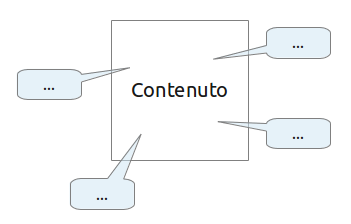
\includegraphics[width=7cm]{img/valore-informativo-contenuto.png}
 \caption{Valore informativo di un contenuto}
 \label{fig:tesi:stage:classificazione:serbatoio-contenuti}
\end{center}
\end{figure}

\subsection{Enciclopedia del sapere}
\label{sec:tesi:stage:criterio-classificazione:enciclopedia}
Attualmente, il limite della piattaforma consiste nell'essere un serbatoio di \textsc{contenuti informativi} disaggregati e priva degli strumenti per classificare e catalogare il sapere custodito conferendovi una struttura ordinata, una sorta di indice in grado di facilitarne la ricerca, il reperimento e la consultazione.

L'obiettivo del criterio di classificazione consiste essenzialmente nel costruire un'enciclopedia del sapere a partire dalle informazioni presenti nei contenuti informativi.

\begin{quotation}
Un'enciclopedia è un'opera letteraria che raccoglie e ordina la sintesi della conoscenza umana in tutti i campi o in un determinato settore. Le enciclopedie sono divise in voci, o lemmi, cui si accede di solito in ordine alfabetico. \cite{wiki:enciclopedia}
\end{quotation}

Il modello concettuale dell'enciclopedia diventa un riferimento utile ad identificare:
\begin{enumerate}
	\item i casi d'uso essenziali concernenti la consultazione del sapere custodito nella piattaforma (ricerca per lemma, argomento o affinità);
	\item gli elementi strutturali del sistema di classificazione (lemmi, accezioni, \ldots);
	\item i requisiti e le specifiche più rilevanti per il criterio di classificazione;
	\item le principali criticità rispetto alla coerenza e consistenza dell'enciclopedia.
\end{enumerate}

\paragraph{Contenuto informativo}
Ciascun contenuto può essere considerato una collezione di frammenti di informazioni (v. figura \ref{fig:tesi:stage:classificazione:serbatoio-contenuti}), che contribuiscono ad arricchire la conoscenza relativa ad uno o più lemmi dell'enciclopedia. Il criterio di classificazione deve quindi tenere traccia della relazione tra contenuti informativi e lemmi per essere in grado di catalogare e ricostruire l'intero sapere disponibile riguardo un certo tema.

\paragraph{Entità}
Nell'ambito della piattaforma, i lemmi vengono definiti entità ($d_i \in D$) e rappresentano elementi concreti (luoghi, persone, eventi, \ldots) o astratti (concetti, temi, \ldots) a cui afferiscono i contenuti.

L'insieme delle entità definite - in un certo istante - all'interno della piattaforma rappresenta il \textsc{dominio della conoscenza} (di seguito per brevità \textsc{dominio}).

\begin{figure}[ht]
	\begin{center}
		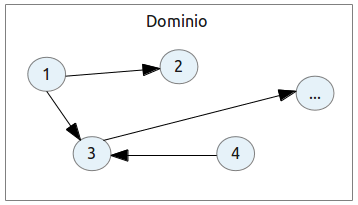
\includegraphics[width=7cm]{img/relazioni-entita.png}
		\label{fig:tesi:stage:fase-uno:entita-relazioni}
		\caption{Relazioni tra le entità del dominio}
	\end{center}
\end{figure}

Così come ciascun lemma di un'enciclopedia contiene spesso riferimenti ad altre voci, che trattano temi specifici o attinenti, nella piattaforma ciascuna entità può riferire o essere riferita da un numero arbitrario di entità distinte e possono esistere riferimenti incrociati, ossia coppie di entità che si citano a vicenda.

Ciò si traduce nel modello relazionale con un vincolo referenziale di tipo molti-a-molti tra le entità, che distingue referenti e riferite e permette di interpretare il dominio $D$ mediante una struttura a grafo orientato ove:
\begin{itemize}
\item ciascun nodo rappresenta un entità;
\item ciascun arco uscente identifica un'\textsc{entità riferita};
\item ciascun arco entrante identifica un'\textsc{entità referente}.
\end{itemize}

\paragraph{Etichette}
Ciascuna entità ha un valore semantico preciso ed univoco, ma dev'essere identificata anche sul piano sintattico mediante un'etichetta ($e_j \in E$), ossia una stringa di lunghezza variabile che consenta agli utenti di riferirla all'interno di ciascun contenuto.

L'insieme di etichette definite in un certo istante costituisce il \textsc{dizionario} della piattaforma.

Il modello illustrato presenta tuttavia due notevoli inconvenienti, che devono essere risolti per soddisfare i requisiti e gli obiettivi fissati: l'ambiguità sintattica e quella semantica.

\subsection{Ambiguità sintattica}
\label{sec:tesi:stage:criterio-classificazione_ambiguità-sintattica}
Nel linguaggio comune, è possibile riferirsi ad una certa entità ($d_i$) con termini o espressioni differenti ($e_{i,j} \in E_i$): la presenza di sinonimi, aventi il medesimo valore semantico ma diversa sintassi, rappresenta un fattore di ambiguità intrinseco e non trascurabile, che trasforma la relazione uno-a-uno tra entità ed etichette in una di tipo uno-a-molti.

\begin{figure}[ht]
	\begin{center}
		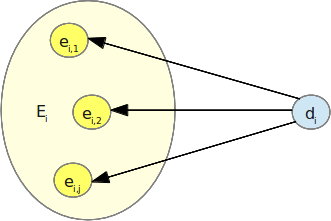
\includegraphics[width=7cm]{img/ambiguita-sintattica.png}
		\label{fig:tesi:stage:fase-uno:ambiguita-sintattica}
		\caption{Ambiguità sintattica di un'entità}
	\end{center}
\end{figure}

Il criterio di classificazione è dunque chiamato a conciliare la possibilità per l'utente di riferirsi ad una certa entità con etichette differenti e l'esigenza di identificarla univocamente nei contenuti informativi.

\paragraph{Sinonimi}
La gestione dei sinonimi di un'entità rappresenta un aspetto cruciale, poiché scegliere tra i possibili sinonimi un'etichetta arbitraria con cui identificare un'entità ed ignorare i rimanenti, pur semplificando il modello, costringerebbe gli utenti a conoscere e ad utilizzare solo quell'etichetta, imponendo una scelta del tutto arbitraria e - in quanto tale - fortemente soggettiva.

Per facilitare la ricerca di un'entità è opportuno includere e conservare nel dizionario tutte le etichette note o utilizzate dagli utenti, così da rendere il sistema sempre più accurato nell'individuare e riconoscere l'entità cui un utente fa riferimento ogni qualvolta utilizza una certa etichetta. Con il passare del tempo, il numero dei sinonimi di ciascuna entità è destinato a crescere grazie al contributo degli utenti, garantendo così una migliore copertura sintattica.

La proliferazione di sinonimi, ossia etichette equivalenti sul piano semantico ma sintatticamente differenti, rischia tuttavia di avere pesanti ripercussioni sull'efficacia del criterio di classificazione e particolarmente sull'efficienza della ricerca: se ai contenuti vengono assegnate delle etichette, reperire tutte e sole le informazioni inerenti una certa entità richiederebbe infatti di cercare riscontri nei contenuti pubblicati per ogni etichetta con cui possa venir riferita.

\paragraph{Contenuti}
A tale inconveniente si pone rimedio facilmente definendo una relazione molti-a-molti tra le entità e i contenuti, che ignori le etichette utilizzate per indicarle.

Così facendo si preserva l'identificazione univoca di ciascuna entità nei contenuti informativi, almeno sul piano semantico, e si guadagna in termini di efficienza.

Si considerino il dizionario $E$ ed il dominio $D$. Il numero medio $\alpha$ di etichette associate a ciascuna entità risulta pari a:\footnote{Poiché la relazione tra etichette ed entità è di tipo uno-a-molti, ciascuna etichetta è associata ad una ed una sola entità. Ne consegue che $P = \{ E_0, E_1, \ldots \}$ è una partizione di $E$, ossia vale $\bigcup E_i = E$ e $\forall A \in P, B \in P: A \neq B \implies A \cap B = \emptyset$.}
\begin{equation} \label{eq:tesi:stage:etichette-per-entità}
\alpha = \frac{\left|E_0\right| + \left|E_1\right| + \ldots}{\left|D\right|} = \frac{\sum{\left|E_i\right|}}{\left|D\right|}
\end{equation}
ove
\begin{equation} \label{eq:tesi:stage:dizionario}
\sum{\left|E_i\right|} = \left|E\right|
\end{equation}

Ciò significa intuitivamente che assegnare ai contenuti un'etichetta arbitraria aumenterebbe di una costante moltiplicativa $\alpha$ la complessità dell'operazione di ricerca, che dovrebbe essere ripetuta per ciascuna delle $\alpha$ etichette anziché per la sola entità corrispondente.\footnote{Si assuma per semplicità che la ricerca verifichi - per ciascun contenuto - quali entità o etichette cercate siano presenti, una per volta, e che la complessità computazionale sia equivalente in entrambi i casi.}

\paragraph{Etichette}
Tuttavia, per riferire un'entità nella piattaforma web occorre caratterizzarla anche sul piano sintattico. Sebbene non vi siano particolari controindicazioni nel permettere all'utente di scegliere l'etichetta da utilizzare nei contenuti pubblicati, si rischia di:
\begin{itemize}
	\item generare ambiguità e confusione tra gli utenti stessi, rendendo poco intuitivo stabilire se due entità citate in due contenuti diversi e con etichette differenti rappresentino effettivamente la stessa;
	\item dover aggiungere alla relazione tra entità e contenuti un'informazione aggiuntiva, ossia l'etichetta scelta per indicarla.
\end{itemize}

Per tale ragione, si individua arbitrariamente - per ciascuna entità $d_i$ - un'\textsc{etichetta primaria} ($e_{i,0} \in E_i$), che la identifica univocamente nell'ambito della piattaforma, mentre le restanti (\textsc{etichette secondarie}) ne vengono considerate sinonimi.

Così facendo si introducono tuttavia alcuni vincoli aggiuntivi sulla relazione, che risulta scissa in due distinte:
\begin{enumerate}
	\item una relazione di tipo uno-a-uno tra l'entità e la corrispondente etichetta primaria;
	\item una relazione uno-a-molti tra l'entità e le etichette secondarie.
\end{enumerate}

\begin{figure}[ht]
	\begin{center}
		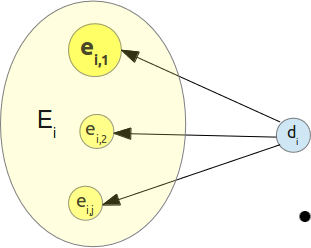
\includegraphics[width=7cm]{img/etichette-primarie-secondarie.png}
		\label{fig:tesi:stage:fase-uno:entita-sintassi-semantica}
		\caption{Etichetta primaria e secondarie}
	\end{center}
\end{figure}

In conclusione, il nodo cruciale della soluzione individuata consiste nel mantenere separato l'aspetto semantico (le entità) da quello sintattico (le etichette): ogni qualvolta l'utente ricerca o assegna un'etichetta ad un contenuto, il sistema traduce il suo ingresso sintattico (l'etichetta) in un'uscita semantica (l'entità corrispondente).

Tale meccanismo è tuttavia soggetto ad alcune complicazioni, dovute all'ambiguità semantica di ciascuna etichetta.

\subsection{Ambiguità semantica}
\label{sec:tesi:stage:criterio-classificazione:ambiguità-semantica}
Riprendendo il modello dell'enciclopedia, si osserva come ciascuna etichetta $e_j$ possa avere svariate \textsc{accezioni} ($a_{j,k} \in A_j$), ciascuna delle quali ne individua un significato differente e si riferisce ad un'entità distinta.

\begin{figure}[ht]
	\begin{center}
		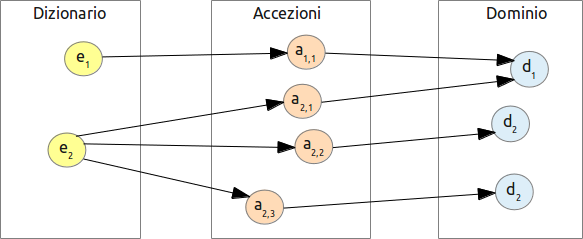
\includegraphics[width=10.5cm]{img/ambiguita-semantica.png}
		\caption{Accezioni di un'etichetta}
		\label{fig:tesi:stage:fase-uno:etichette-accezioni}
	\end{center}
\end{figure}

Sebbene la natura tematica della piattaforma tenda a mitigare la presenza di etichette aventi accezioni multiple, tale eventualità non può essere esclusa e dev'essere dunque opportunamente gestita.

Occorre innanzi tutto rivedere la relazione uno-a-molti tra entità ed etichette, che diventa di tipo molti-a-molti e per cui vale la proprietà illustrata di seguito.

Siano $a_{j,k}$ e $a_{j,k'}$ accezioni distinte di un'etichetta $e_j$ e sia definita la funzione
\begin{equation}
f(a_{j,k}): A_j \rightarrow D
\end{equation}
che restituisce l'entità $d_i$ riferita dall'accezione $a_{j,k}$. Allora
\begin{equation}
a_{j,k} \neq a_{j,k'} \implies f(a_{j,k}) \neq f(a_{j,k'})
\end{equation}

\begin{figure}[ht]
	\begin{center}
		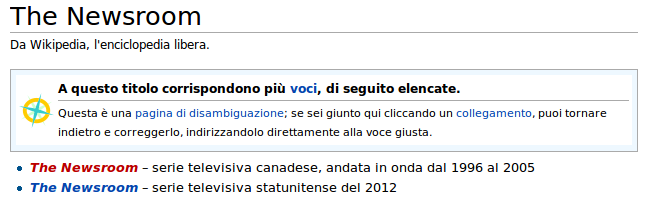
\includegraphics[width=12cm]{img/disambigua.png}
		\label{fig:tesi:stage:classificazione:disambiguazione}
		\caption{Pagina di disambiguazione \cite{wiki:disambigua}}
	\end{center}
\end{figure}

L'equazione \ref{eq:tesi:stage:etichette-per-entità} conserva la propria validità, mentre la \ref{eq:tesi:stage:dizionario} dev'essere modificata per riflettere la differente molteplicità della suddetta relazione, ossia che ciascuna etichetta riferisce una o più entità:
\begin{equation}
	\sum{\left|E_i\right|} = \sum{\left|B_i\right|} = \left|A\right| =	\sum{\left|A_j\right|} \geq \left|E\right|
\end{equation}

%La prima uguaglianza esprime una banale identità tra le etichette di un'entità e  e le accezioni corrispondenti; la seconda discende dal fatto che $P' = {B_1,B_2,\ldots}$ rappresenta una partizione di $A$ rispetto alle entità, mentre la successiva uguaglianza si deduce analogamente dal fatto che $P''={A_1, A_2, \ldots}$ è anch'essa partizione di $A$ (rispetto alle etichette); l'ultima disuguaglianza si deduce osservando che $\forall j \left|A_j\right| \geq 1$, ossia per ciascuna etichetta del dizionario esiste almeno un'accezione.

A ciascuna entità continuano ad essere associate una e una sola etichetta primaria e un numero arbitrario (anche nullo) di etichette secondarie. Ove ciascuna etichetta può riferirsi a diverse entità, tale distinzione varia a seconda dell'accezione considerata, poiché la medesima etichetta può essere primaria rispetto ad un entità e secondaria rispetto ad un'altra.

Per preservare i suddetti vincoli sulle relazioni tra etichette ed entità, si classificano le accezioni in \textsc{chiave} ($a_{j,0}$) o \textsc{sinonimiche} ($a_{j,1},\ldots$), a seconda che l'etichetta risulti rispettivamente primaria o secondaria per l'entità corrispondente. In questo modo si riesce a trasferire tale distinzione dalle etichette alle accezioni, preservando la percezione della relazione dal punto di vista dell'entità.

\begin{figure}[ht]
	\begin{center}
		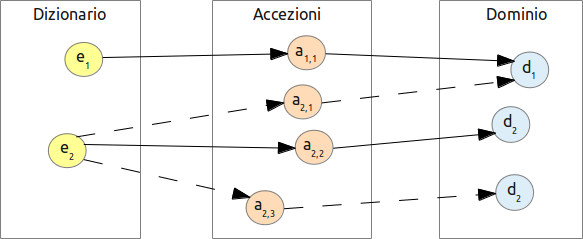
\includegraphics[width=10.5cm]{img/accezioni-chiave-sinonimiche.png}
		\caption{Accezioni chiave e sinonimiche}
		\label{fig:tesi:stage:fase-uno:accezioni-chiave-sinonimiche}
	\end{center}
\end{figure}

A risentire maggiormente dell'esistenza delle accezioni è il processo di ricerca di un'entità $d_i$ a partire da un'etichetta $e_j$: se $\left|A_j\right|\geq 2$ l'identificazione dell'entità richiede - da parte dell'utente - la selezione di un'accezione $a_{j,k} \in A_j$ tra le $\left|A_j\right|$ disponibili per indicare esplicitamente l'entità cui fa riferimento.

\subsection{Modello relazionale}

\begin{figure}[ht]
	\begin{center}
		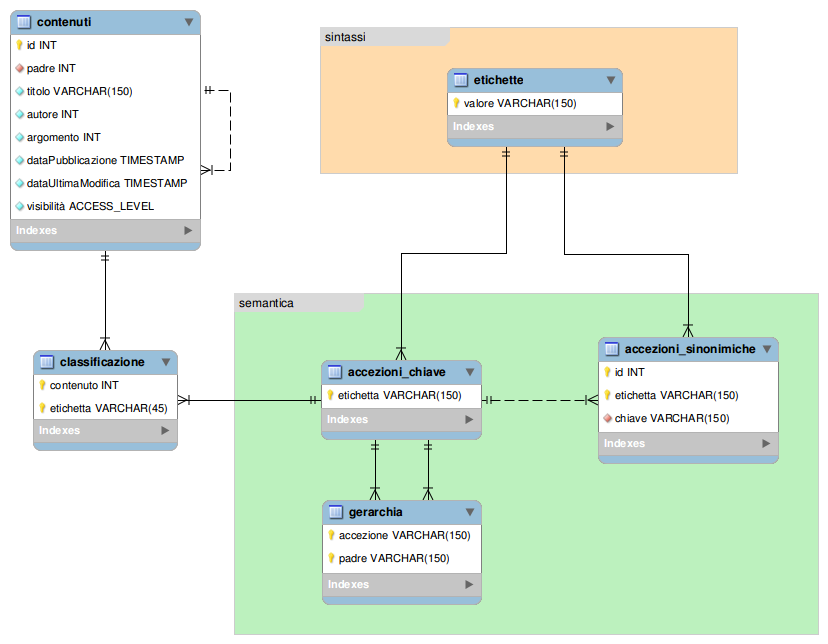
\includegraphics[width=12cm]{img/modello-er.png}
		\caption[Modello relazionale]{Modello relazionale del criterio di classificazione}
		\label{fig:tesi:stage:er:modello}
	\end{center}
\end{figure}

Al termine della fase progettuale, si rende necessario modificare il modello relazionale della piattaforma per integrare le informazioni addizionali legate al nuovo criterio di classificazione.

Rispetto all'immagine \ref{fig:tesi:stage:er:modello}, la sola tabella \textsf{contenuti} risulta importata dal modello relazionale della piattaforma per evidenziare alcuni vincoli fondamentali. Le rimanenti sono organizzate in tre \textit{layer} (\textsf{contenuti}, \textsf{semantica} e \textsf{sintassi}) per chiarirne il ruolo all'interno del sistema di classificazione.

\paragraph{Etichette}
Le etichette sono rappresentate mediante la tabella \textsf{etichette} e sono identificate univocamente dalla stringa associata, che rappresenta l'attributo \textsf{etichette.valore}. Tale scelta risponde alla naturale identificazione dell'etichetta nella sequenza di caratteri corrispondente, costituisce una garanzia contro la presenza di duplicati e consente di recuperare il valore dell'etichetta primaria di un'entità senza dover effettuare un'operazione di \textit{join} tra le tabelle \textsf{entita} ed \textsf{etichette}.

\paragraph{Accezioni}
Le accezioni rappresentano un legame univoco tra le etichette e le entità e possono essere di tipo chiave o sinonimico. Esse non presentano attributi propri significativi, ma prevedono tre vincoli referenziali:
\begin{enumerate}
\item a ciascuna entità è associata una e una sola accezione chiave (relazione uno-a-uno), che ne identifica l'etichetta primaria;
\item a ciascuna entità sono associate $0\ldots n$ accezioni sinonimiche (relazione uno-a-molti), che rappresentano i sinonimi dell'etichetta primaria;
\item ciascuna etichetta possiede $0\ldots n$ accezioni (relazione uno-a-molti).
\end{enumerate}

\begin{figure}[ht]
	\begin{center}
		
\includegraphics{img/placeholder.png}
		\caption{Modello ad oggetti delle accezioni}
		\label{fig:tesi:stage:er:accezioni}
	\end{center}
\end{figure}

Ne consegue che sia la superclasse (\textsf{accezioni}) sia le sottoclassi \linebreak(\textsf{accezioni\textunderscore chiave} e \textsf{accezioni\textunderscore sinonimiche}) presentano dei vincoli referenziali; in particolare, la presenza delle prime due relazioni costringe a distinguere - dal punto di vista dell'entità - tra accezioni chiave e sinonimiche.

Per modellare tale scenario vengono presi in considerazione tre possibili approcci:
\begin{description}
\item[Tabella unica] \hfill \\
La tabella unica ben si adatta a gestire l'assenza di attributi propri per le sottoclassi e ad esprimere i vincoli referenziali che coinvolgono la superclasse, ma non è in grado di esprimere e adeguatamente rappresentare quelli coinvolgenti le sottoclassi.
\item[Partizionamento orizzontale] \hfill \\
Il partizionamento orizzontale riesce a modellare i vincoli referenziali delle sottoclassi, ma non quello della superclasse, e genera due classi aventi i medesimi attributi.
\item[Partizionamento verticale] \hfill \\
Il partizionamento verticale consente di modellare correttamente tutti e tre i vincoli referenziali, relativi sia alla superclasse sia alle sottoclassi. Tuttavia si rende più complesso modificare il tipo di un'accezione e si introduce l'esigenza di un'operazione \textit{join} per recuperare la lista completa delle accezioni, pur non possedendo le sottoclassi attributi propri.
\end{description}

\pagebreak
A seguito di alcune osservazioni si decide di adottare la soluzione della tabella unica:
\begin{itemize}
\item la distinzione tra etichette chiave e sinonimiche ha rilevanza essenzialmente dal punto di vista della classe \textsf{entita};
\item il vincolo referenziale tra \textsf{etichette} ed \textsf{accezioni} suggerisce che la distinzione di cui al punto precedente sia irrilevante dal punto di vista delle etichette, ragion per cui risulta utile mantenere tutte le accezioni nella medesima tabella.\footnote{Si consideri ad esempio il caso d'uso della ricerca di un'entità a partire da un'etichetta, ove occorre recuperare la lista completa delle relative accezioni.}
\item le sottoclassi non hanno attributi propri, per cui il partizionamento verticale e orizzontale sono ritenute soluzioni inadeguate.
\end{itemize}

Il soddisfacimento delle condizioni richieste viene raggiunto eliminando qualsiasi riferimento al tipo dell'accezione nella classe \textsf{accezioni} e modellando direttamente la relazione uno-a-uno tra le entità e le relative etichette primarie mediante un vincolo referenziale di chiave esterna nella classe \textsf{entita} (\textsf{entita.etichetta}), che identifica la corrispondente etichetta primaria (\textsf{etichette.valore}). Così facendo si riescono ad esprimere tutti i vincoli referenziali senza la necessità di definire le sottoclassi.

%--------
% SECTION
%--------
\section{Filtri di ricerca}
\label{sec:tesi:stage:gui:filtri}

\subsection{Introduzione}
La seconda fase dell'attività di stage consiste nell'analisi e nella progettazione di un'interfaccia grafica per la consultazione dei risultati di una ricerca sui contenuti informativi, che sfrutti il criterio di classificazione definito in precedenza e permetta all'utente di:
\begin{enumerate}
	\item impostare i parametri iniziali di ricerca (parole chiave, ambito);
	\item modificare la lista delle entità cercate mediante sostituzione o eliminazione;
	\item filtrare i risultati di ricerca in accordo a criteri di classificazione o proprietà dei contenuti;
	\item consultare - in forma grafica o testuale - le proprietà fondamentali, i metadati di classificazione e i legami tra i contenuti;
	\item mostrare la \textsc{discussione} associata ad un contenuto informativo;
	\item impostare i filtri personalizzati (solo per utenti autenticati).
\end{enumerate}

Nella fase di progettazione dell'interfaccia grafica devono essere tenuti in debita considerazione alcuni requisiti di qualità desiderabili:
\begin{itemize}
  \item deve risultare intuitiva e facilmente utilizzabile da qualsiasi categoria di utenti, a prescindere dal livello di esperienza e dalla familiarità con piattaforme web esistenti (\textit{chat}, \textit{forum}, \textit{social network}, \ldots);
  \item dev'essere fruibile dal maggior numero possibile di dispositivi (\textit{computer}, \textit{tablet}, \textit{smartphone}, \ldots), ciascuno secondo le peculiari modalità di interazione;
  \item deve rappresentare in maniera ordinata ed efficace le informazioni, a prescindere dal numero di contenuti caricati.
\end{itemize}

\subsection{Parametri}
La progettazione dei filtri di ricerca richiede innanzi tutto di scegliere i criteri di classificazione e le proprietà dei contenuti informativi (di seguito \textsc{parametri}) utilizzabili in combinazione ad un filtro.

Il requisito obbligatorio consiste nell'essere definiti su un insieme $U$ di possibili valori $u \in U$, ciascuno dei quali - in un dato istante - dev'essere ammissibile ($u \in U_A$) o bloccato ($u \in U_B$). Deve quindi valere in ogni istante che $U_A \cap U_B = \emptyset$ e $U_A \cup U_B = U$.

Inizialmente tutti i valori relativi ad un certo parametro sono ammessi, ossia $U_A = U$ e $U_B = \emptyset$: l'azione dell'utente altera tale suddivisione dell'insieme $U$ bloccando un valore, autorizzandolo o azzerando il filtro, ossia rendendo ammissibili tutti i valori ($U_A = U$).

\paragraph{Soddisfacibilità}
Un contenuto informativo, incluso tra i risultati di ricerca, viene quindi visualizzato se e solo se il valore di ciascun parametro soddisfa il filtro associato.

A seconda che i contenuti assumano - per un dato parametro - un singolo valore (autore, data di pubblicazione, \ldots) o una lista (emozioni, etichette, intenzioni, \ldots), il filtro è soddisfatto se e solo se:
\begin{itemize}
\item il valore assunto è ammissibile (valore singolo);
\item almeno uno dei valori assunti è ammissibile (valori multipli).
\end{itemize}

Al termine dell'analisi viene redatta una lista completa dei parametri soddisfacenti il requisito iniziale, visibile nella tabella \ref{tab:tesi:stage:parametri-filtri} (tra parentesi si riporta il nome della classe corrispondente, ove disponibile).\footnote{Il termine \textsc{etichette} riportato nella tabella designa in seguito il criterio di classificazione illustrato nella sezione \ref{sec:tesi:stage:criterio-classificazione}. L'espressione \textit{Data di pub.} è un'abbreviazione usata di seguito per indicare la data di pubblicazione.}
\begin{table}[ht]
\centering
\begin{tabular}{|l|l|}
\hline
\textsc{Proprietà} & \textsc{Criteri di classificazione} \\ \hline
Autore (\textsf{User}) & Argomento (\textsf{Topic})\\
Data di pub. (\textsf{Date}) & Emozioni (\textsf{Emotion}) \\
Tipo (\textsf{Type}) & Etichette (\textsf{Entity}) \\
Giudizi (\textsf{Rating}) & Interessi (\textsf{Interest}) \\
& Intenzioni (\textsf{Intention}) \\ \hline
\end{tabular}
\caption{Lista dei parametri per i filtri di ricerca}
\label{tab:tesi:stage:parametri-filtri}
\end{table}

\subsection{Classi di filtri}
Per identificare i requisiti e i casi d'uso correlati ai filtri di ricerca risulta conveniente classificarli in relazione a:
\begin{itemize}
  \item la natura dell'insieme $U$ (ordinato, finito, \ldots);
  \item le modalità d'interazione dell'utente (selezione di un intervallo, impostazione di una soglia, \ldots), che determinano i sottoinsiemi $U_A$ e $U_B$.
\end{itemize}

L'analisi si conclude con l'individuazione di quattro classi di filtri di ricerca, illustrate di seguito.

\paragraph{A lista di valori}
Il filtro a lista di valori consente di autorizzare o bloccare selettivamente ciascun elemento $u \in U$. I casi d'uso includono:
\begin{itemize}
	\item la consultazione della lista dei valori ammessi ($U_A$);
	\item la consultazione della lista dei valori bloccati ($U_B$);
	\item l'autorizzazione di un valore;
	\item il blocco di un valore;
	\item l'azzeramento del filtro ($U_A = U$ e $U_B = \emptyset$).
\end{itemize}
	
\paragraph{A soglia di valore}
Nel filtro a soglia di valore l'insieme $U$ è ordinato e contiene un elemento minimo $min \in U$ ed uno massimo $max \in U$.

L'utente può scegliere arbitrariamente un valore $x$, purché soddisfi la condizione $min \leq x \leq max$. L'insieme dei valori ammissibili risulta così definito: $U_A = \lbrace u : u \geq x, u \in U\rbrace$.

\paragraph{Ad intervallo}
Nel filtro ad intervallo l'insieme $U$ è ordinato e contiene un elemento minimo $min \in U$ ed uno massimo $max \in U$.

L'utente può liberamente selezionare l'estremo inferiore ($inf \in U$) e superiore ($sup\in U$) dell'intervallo, purché sia soddisfatta la seguente catena di disuguaglianze: $min \leq inf \leq sup \leq max$.

L'insieme dei valori ammissibili risulta ovviamente $U_A = \lbrace u \in U : inf \leq u \leq sup \rbrace$.

I casi d'uso annoverano:
\begin{itemize}
	\item la selezione del valore minimo $inf$;
	\item la selezione del valore massimo $sup$.
	\item la selezione di un valore esatto ($inf = sup$).
\end{itemize}

\paragraph{Ad interruttore}
Il filtro ad interruttore consente all'utente di scegliere se applicare o meno ai risultati di ricerca il filtro corrispondente, che può essere di un tipo qualsiasi tra quelli descritti in precedenza.

I casi d'uso prevedono solamente:
\begin{itemize}
	\item l'attivazione del filtro;
	\item la disattivazione del filtro.
\end{itemize}

\begin{table}[ht]
\centering
\begin{tabular}{|l|l|l|l|}
\hline
\textsc{Lista di valori} & \textsc{Soglia di valore} & \textsc{Intervallo} & \textsc{Interruttore}\\ \hline
Autore & Giudizi & Data di pub. & Interessi \\
Argomento & & & \\
Emozioni & & & \\
Etichette & & & \\
Intenzioni & & & \\
Tipo & & & \\ \hline
\end{tabular}
\caption{Elenco dei parametri per i filtri di ricerca, suddivisi per tipo.}
\label{tab:tesi:stage:parametri-filtri-tipo}
\end{table}
	
\subsection{Progettazione}
La fase di progettazione deve integrare nell'architettura \underline{MVC} della piattaforma le classi e i parametri dei filtri di ricerca; il risultato finale è mostrato nella tabella \ref{tab:tesi:stage:design:filter-factory}.

\paragraph{Model}
 Ciascun tipo di filtro di ricerca è rappresentato dalla classe corrispondente (v. figura \ref{fig:tesi:stage:design:model-filter-classi}), che implementa un'interfaccia standard (\textsf{Filter}) per ridurre l'accoppiamento con le altre componenti e facilitare l'estendibilità del sistema (aggiunta di nuovi tipi di filtri, \ldots):
  \begin{itemize}
    \item \textsf{FList} (a lista di valori);
    \item \textsf{FRange} (ad intervallo);
    \item \textsf{FSwitch} (ad interruttore);
    \item \textsf{FValue} (a soglia di valore).
  \end{itemize}
  
\begin{figure}[ht]
	\begin{center}
		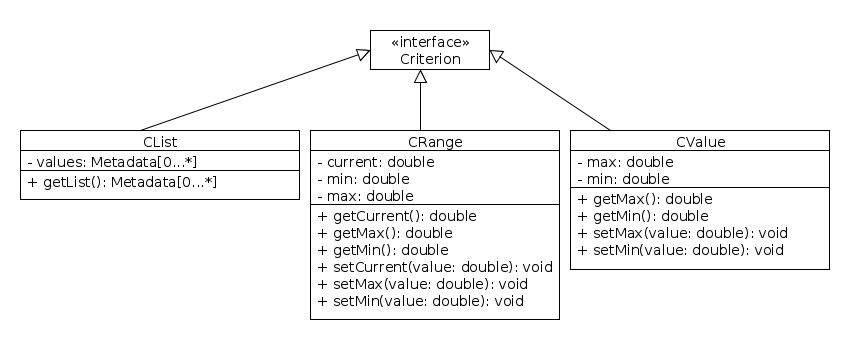
\includegraphics[width=12cm]{img/model_filter.png}
		\caption{Diagramma delle classi per il package \textit{model.filter}}
		\label{fig:tesi:stage:design:model-filter-classi}
	\end{center}
\end{figure}

  A parità di classe del filtro, i parametri differiscono per le specifiche dell'insieme $U$, in particolare per la \textsc{sorgente} (statica o dinamica) ed il \textsc{tipo} (emozioni, intenzioni, etichette, \ldots) di dati gestiti.
  
  Ciascuna classe riportata nella tabella \ref{tab:tesi:stage:parametri-filtri} rappresenta - a livello di tipo - il corrispondente parametro (un generico insieme $U$) mentre - a livello di istanze - ciascuno dei possibili valori ($u \in U$).

Per rendere le classi dei filtri polimorfe rispetto ai parametri, ossia per facilitare l'aggiunta, l'aggiornamento e la rimozione di questi ultimi, si definisce una classe astratta (\textsf{Metadata}), che tutte le suddette classi devono estendere. Essa include un metodo astratto (\textsf{getValueList}) da ridefinire per gestire opportunamente l'approvvigionamento dell'insieme dei valori $u \in U$, sia che si tratti di una lista statica (tipo, argomento, \ldots) o dinamica (autore, data di pubblicazione, \ldots), ossia ricavata dai risultati di ricerca. Nel primo caso la lista di valori può essere memorizzata direttamente in un campo dati statico della classe.

I filtri vengono quindi creati a partire da una lista di valori, collezione di istanze di una sottoclasse concreta di \textsf{Metadata}: per favorire il disaccoppiamento si introducono alcune classi aggiuntive (v. figura \ref{fig:tesi:stage:design:model-criteria-classi}), che incapsulano tali valori e li rendono accessibili mediante un'interfaccia standard:
\begin{itemize}
  \item \textsf{CList} (criterio a lista di valori);
  \item \textsf{CRange} (criterio ad intervallo);
  \item \textsf{CValue} (criterio a soglia di valore).
\end{itemize}

Questa soluzione offre la possibilità di inizializzare un filtro ad interruttore con qualsiasi tipo di criterio, nascondendone così le specifiche alle classi che ne gestiscono solamente lo stato di attivazione (\textsf{FSwitch} e \textsf{FVSwitch}).
	
\begin{figure}[ht]
\begin{center}
	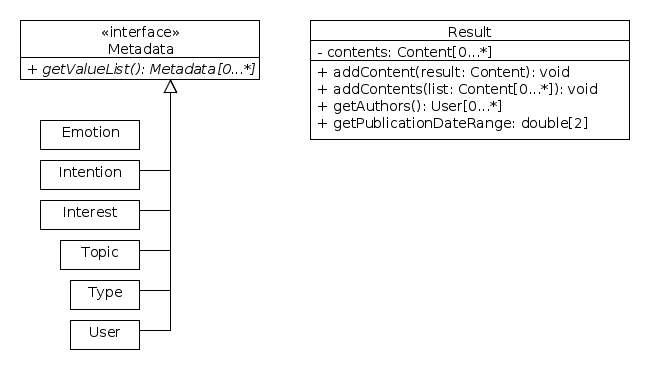
\includegraphics[width=12cm]{img/model_criteria.png}
	\caption{Diagramma delle classi per il package \textit{model.criteria}}
	\label{fig:tesi:stage:design:model-criteria-classi}
\end{center}
\end{figure}

\paragraph{View}
	Ciascun tipo di filtro richiede un componente grafico differente, che metta a disposizione dell'utente gli strumenti e le opzioni adeguate per consentire un'interazione coerente rispetto a quanto previsto dai rispettivi casi d'uso:
	\begin{itemize}
	  \item \textsf{FVList} (filtro a lista di valori);
	  \item \textsf{FVRange} (filtro ad intervallo);
	  \item \textsf{FVSwitch} (filtro ad interruttore);
	  \item \textsf{FVValue} (filtro a soglia di valore).
	\end{itemize}
Ciascuna classe implementa un'interfaccia standard (\textsf{ViewFilter}) e viene istanziata con un corrispondente oggetto di tipo \textsf{Filter}. Per assicurare che il tipo dinamico dell'oggetto sia coerente rispetto al tipo statico del componente grafico (v. tabella \ref{tab:tesi:stage:design:filter-factory}) il costruttore di ciascuna classe considerata si aspetta un argomento avente tipo statico corrispondente alla sottoclasse concreta di \textsf{Filter}, che modella il filtro corrispondente.

\begin{figure}[ht]
\begin{center}
	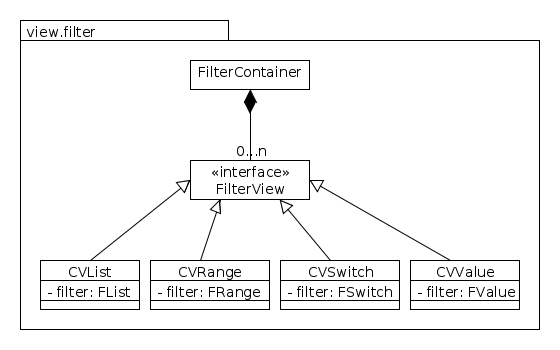
\includegraphics[width=8cm]{img/view_filter.png}
	\caption{Diagramma delle classi per il package \textit{view.filter}}
	\label{fig:tesi:stage:design:view-filter-classi}
\end{center}
\end{figure}

\paragraph{Controller}
Ciascun tipo di filtro prevede diverse modalità d'interazione, che richiedono di essere gestite mediante altrettante classi del \textsf{controller}

\paragraph{Abstract Factory}
Per assicurare la corretta combinazione di istanze delle classi (v. tabella \ref{tab:tesi:stage:design:filter-factory}) si ricorre al \textit{design pattern} \textit{Abstract Factory}, a cui sono note le corrette combinazioni di oggetti da utilizzare e che permette così di nascondere i dettagli relativi alle classi effettivamente istanziate durante il processo di creazione di un filtro.

\begin{table}
	\centering
	\begin{tabular}{|l|c|c|c|c|c|}
	\hline
	 & \textsf{Metadata} & \textsf{Criterion} & \textsf{Filter} & \textsf{FilterController} & \textsf{FilterView} \\ \hline
	Argomento & \textsf{Topic} & \textsf{CList} & \textsf{FList} & \textsf{FCList} & \textsf{FVList} \\ \hline
	Autore & \textsf{User} & \textsf{CList} & \textsf{FList} & \textsf{FCList} & \textsf{FVList} \\ \hline
	Data di pub. & \textsf{Date} & \textsf{CRange} & \textsf{FRange} & \textsf{FCRange}& \textsf{FVRange} \\ \hline
	Emozioni & \textsf{Emotion} & \textsf{CList} & \textsf{FList} & \textsf{FCList} & \textsf{FVList} \\ \hline
	Giudizi & \textsf{Rating} & \textsf{CValue} & \textsf{FValue} & \textsf{FCValue} & \textsf{FVValue} \\ \hline
	Intenzioni & \textsf{Intention} & \textsf{CList} & \textsf{FList} & \textsf{FCList} & \textsf{FVList} \\ \hline
	Interessi & \textsf{Interest} & \textsf{CList} & \textsf{FSwitch} & \textsf{FCSwitch} & \textsf{FVSwitch} \\ \hline
	Tipo & \textsf{Type} & \textsf{CList} & \textsf{FList} & \textsf{FCList} & \textsf{FVList} \\ \hline
	\end{tabular}
	\caption{Riepilogo delle classi gestite dall \textit{design patter} \textit{Abstract Factory}}
	\label{tab:tesi:stage:design:filter-factory}
\end{table}

	\chapter{Valutazioni finali}
\label{ch:tesi:valutazioni}

\section{Obiettivi}
Nel corso dello stage sono state svolte due attività correlate, ma differenti in merito al tipo di impegno e di competenze richieste:
\begin{enumerate}
  \item lo sviluppo di un criterio di classificazione aggiuntivo per catalogare il sapere custodito nei contenuti pubblicati dagli utenti nella piattaforma;
  \item l'analisi e la progettazione di un'interfaccia grafica per la consultazione dei risultati di una ricerca sui contenuti informativi.
\end{enumerate}

La progettazione del criterio di classificazione ha richiesto nella fase iniziale dello stage un'attività di ricerca riguardante lo stato dell'arte dei sistemi di classificazione attualmente adottati nelle principali piattaforme di condivisione di contenuti:
\begin{itemize}
  \item blog (\textit{Drupal}, \textit{Wordpress});
  \item forum;
  \item social network (\textit{Facebook}, \textit{Twitter}).
\end{itemize}

I risultati di questa analisi hanno consentito di conoscere i principali meccanismi di catalogazione delle informazioni, di evidenziarne le principali analogie e differenze e di coglierne i punti di forza e di debolezza: a partire da queste informazioni ho inteso affrontare lo sviluppo di un criterio di classificazione, che riuscisse a coniugare - nella soluzione più semplice e adatta alla piattaforma \textit{Social (Life) Shuttle} - gli aspetti essenziali riuscendo al contempo a superarne i limiti evidenziati.

I principali dubbi e criticità sono emersi al momento di valutare l'interazione dell'utente in particolari scenari e casi d'uso: sebbene il criterio di classificazione risolva i problemi legati alle ambiguità sintattiche e semantiche, occorre considerare che la distinzione tra sintassi e semantica comporta la necessità di inviduare esplicitamente le relazioni tra entità del dominio ed etichette del dizionario, al fine di garantire la consistenza e coerenza del criterio stesso, ogni qualvota si definisce una nuova entità, si crea una nuova etichetta o si aggiunge un'accezione ad un'etichetta esistente.

In tali frangenti occorre individuare meccanismi che siano in grado di fornire aiuto e assistenza agli utenti nel processo di individuazione di tali legami o provvedere ad effettuare un controllo a posteriori finalizzato ad assicurare - con il miglior margine possibile - la consistenza del dizionario e del dominio, la correttezza o l'assenza dei suddetti legami tra entità ed etichette.

Un esempio emblematico riguarda l'individuazione dell'entità associata ad una nuova etichetta utilizzata da un utente: in certi casi, ad esempio con i nomi propri, possono esistere molteplici varianti, inclusi nomi d'arte o soprannomi generici che differiscono a volte marginalmente a volte sensibilmente sul piano sintattico, e occore individuare la correlazione esistente sul piano semantico.

Data la natura complessa del problema, queste criticità sono state raccolte e segnalate ai restanti membri del team e saranno oggetto di indagini da parte di persone qualificate. Nell'attesa si intende dotare ogni declinazione della piattaforma di un dizionario delle espressioni e un dominio degli argomenti principali, in modo da fornire una solida base rispetto alla quale catalogare e classificare le informazioni che saranno presenti nei contenuti pubblicati.  

La fase di analisi dei requisiti ha approfondito le modalità d'interazione dell'utente generico con il sistema a partire dai requisiti essenziali illustrati nella sezione \ref{sec:tesi:progetto:requisiti:interfaccia-grafica}, riuscendo ad individuare requisiti impliciti e caratteristiche funzionali inizialmente non preventivate.

La decisione, presa di comune accordo con il referente aziendale, di demandare la valutazione delle tecnologie di sviluppo al momento in cui le specifiche della piattaforma e le esigenze tecniche dell'interfaccia fossero più stabili e definite ha richiesto uno sforzo aggiuntivo di astrazione per quanto concerne la progettazione della soluzione, ma al contempo ha rappresentato uno spunto di riflessione per comprendere con maggior chiarezza il ruolo e l'identità della fase stessa nel ciclo di vita del software.

Nell'ambito dell'agnosticismo tecnologico, le attività si sono focalizzate sull'architettura e sulla presentazione dell'interfaccia grafica, fornendo ove possibile e utile delle linee guida o delle specifiche dettagliate riguardo approcci risolutivi (\textit{design pattern}) o componenti di particolare interesse o rilevanza per il progetto, al fine di chiarire l'impianto progettuale.

Le soluzioni concepite hanno comunque tenuto conto delle esigenze di adattabilità a cambiamenti ed evoluzioni del sistema, incluse l'estensione o integrazione di funzionalità esistenti.

\section{Competenze professionali}
Le attività di stage si inseriscono nell'ambito di un percorso di collaborazione con l'azienda \textit{Sintesi Sas}, iniziato in occasione dell'iniziativa \textit{Mimprendo} promossa da \textit{Confindustria Padova}, che mi ha permesso di seguire il percorso evolutivo del progetto \textit{Social (Life) Shuttle} sin dai primi albori ed ha rappresentanto un'opportunità di crescita professionale molto rilevante.

Sin dalle attività precedenti ma particolarmente nel corso dello stage ho potuto apprezzare gli enormi benefici - in termini di competenze professionali acquisite - derivanti dall'operare all'interno di un progetto caratterizzato da un forte carattere multidisciplinare: il team di progetto include infatti figure provenienti da svariati settori professionali (psicologia, sociologia, marketing, economia, informatica, ingegneria, \ldots), che collaborano attivamente e a stretto contatto integrando le reciproche conoscenze e competenze.

Nel corso dell'attività di stage ho avuto occasione di confrontarmi con queste figure, da cui ho appreso informazioni che mi hanno consentito di svolgere le attività previste nel modo migliore e che mi hanno fatto comprendere come il successo di un progetto non possa in alcun modo prescindere dal contributo di competenze professionali diverse.

L'analisi, la progettazione e lo sviluppo della piattaforma \textit{Social (Life) Shuttle} non si limitano a considerare i soli aspetti tecnici o tecnologici nella concezione e nella valutazione delle soluzioni da adottare nell'intero ciclo di vita del software, ma cercano di comprendere ed intepretare le esigenze degli utenti e le dinamiche sociali. In questa piattaforma di socializzazione e di condivisione della conoscenza la tecnologia è diventata non il fine, bensì il mezzo attraverso il quale si cerca di concretizzare un certo tipo di esperienza virtuale (e non).

Durante la fase di integrazione del criterio di classificazione nel modello relazionale della piattaforma le competenze acquisite in ambito universitario mi hanno permesso di individuare soluzioni semplici ma efficaci, che sono state accolte e giudicate positivamente dal team di progetto. Le principali difficoltà incontrate riguardano l'integrazione della propria soluzione nel modello relazionale esistente in maniera coerente e collaborativa, essendo diverse persone impegnate, seppur su fronti diversi, alla modifica e all'aggiornamento dello stesso.

Le attività previste per la seconda fase dello stage sono state caratterizzate solo in minima parte da attività di ricerca, integrata in molti aspetti da indagini di carattere sociologico. Queste, seppur preliminari, hanno rappresentato un contributo cruciale nel processo di identificazione e comprensione delle variegate esigenze di utenti con profili esperienziali diversificati e di valutazione delle scelte progettuali effettuate.

La maggior parte del tempo a disposizione è stato speso per effettuare l'analisi dei requisiti, che ha permesso di delineare i casi d'uso degli utenti e individuare alcuni requisiti fondamentali: in questa fase si è rivelata decisiva per lo svolgimento delle attività previste in modo da rispettare il piano di lavoro un'organizzazione del lavoro e una metodologia acquisiti e maturati durante la carriera universitaria.

La documentazione prodotta, in particolare, è stata giudicata assai favorevolmente per la completezza e l'organicità con cui sono stati presentati e illustrati in dettaglio i risultati del lavoro svolto nell'arco delle varie settimane.

\section{Stage e università}
Sebbene la formazione universitaria mi abbia consentito di superare piuttosto agevolmente le sfide e le difficoltà incontrate lungo il percorso di stage, grazie alle conoscenze e alle metodologie di lavoro acquisite, il principale fattore di novità riscontrato nell'ambito del progetto \textit{Social (Life) Shuttle} è rappresentato dal taglio fortemente multidisciplinare, che obbliga a rivedere un modello di pensiero ed una \textit{forma mentis} principalmente focalizzate sull'aspetto tecnico e tecnologico del prodotto.

Sin dalle prime comunicazioni con il referente aziendale, mi è risultato chiaro come l'attitudine a pensare in termini multidisciplinari fosse necessaria per comprendere lo spirito e gli obiettivi del progetto: maturato nel corso dei mesi, grazie al dialogo e alla collaborazione con gli altri membri del team di progetto, tale approccio ha rappresentato un elemento cruciale per integrarsi con successo nel e comprenderne a fondo le reali esigenze ed il genuino spirito.

Durante l'attività di stage, si sono rivelati fondamentali per il conseguimento degli obiettivi fissati un'approccio sistematico e organizzato alle fasi di analisi e progettazione dell'interfaccia, frutto degli insegnamenti impartiti nel corso di \textit{Ingegneria del Software} e dell'esperienza maturata durante l'attività di progetto collegata.

L'esperienza di stage ha consentito di rivalutare il ruolo decisivo svolto da attività in precedenza considerate di minor rilevanza come la pianificazione accurata delle attività e la documentazione dei risultati ottenuti: in diversi frangenti la redazione stessa della documentazione mi ha consentito di rilevare incogruenze, criticità o aspetti non sufficientemente approfonditi, permettendomi così di apportare tempestivamente correttivi e miglioramenti.

La varietà di tecnologie, linguaggi e prodotti con cui mi sono misurato durante l'intera esperienza nell'ambito del progetto \textit{Social (Life) Shuttle} ha rafforzato via via la convinzione che le competenze metodologiche e la \textit{forma mentis} rivestano un ruolo decisamente più rilevante rispetto alla conoscenza di linguaggi o tecnologie e meritino di essere affrontate sin dai primi corsi di laurea per stimolare un approccio organizzato e multidisciplinare al lavoro.
%- il percorso continua a livello professionale


	%=========
	% APPENDIX
	%=========
	\appendix
		%********************************************************************
% Appendix
%*******************************************************
% If problems with the headers: get headings in appendix etc. right
%\markboth{\spacedlowsmallcaps{Appendix}}{\spacedlowsmallcaps{Appendix}}
\chapter{Glossario}
\label{ch:tesi:appendice:glossario}

\section*{B}
\paragraph{Bitbucket - \url{https://bitbucket.org/}} \hfill \\
Piattaforma web per la gestione delle attività di progetto con supporto a strumenti di controllo di versione distribuito.

\section*{C}
\paragraph{CamelCase} \hfill \\
Convenzione per la scrittura di espressioni composte unendo le parole tra loro e mantenendo ciascuna iniziale in maiuscolo.

\section*{G}
\paragraph{gedit - \url{http://projects.gnome.org/gedit/}} \hfill \\
Editor di testo ufficiale dell'ambiente desktop GNOME.
%\paragraph{Gruppi di acquisto} \hfill \\
%Insieme (stabile o provvisorio) di consumatori che acquista mediante ordine collettivo un consistente numero di beni direttamente dal produttore, spesso per conseguire prezzi vantaggiosi o ammortizzare eventuali spese accessorie.

\section*{L}
\paragraph{LaTeXila - \url{http://projects.gnome.org/latexila/}} \hfill \\
Editor LaTex integrato per l'ambiente desktop GNOME.
\paragraph{LibreOffice Calc - \url{http://www.libreoffice.org/}} \hfill \\
Applicazione per fogli di calcolo della suite di produttività \textit{LibreOffice}.

\section*{M}
\paragraph{Mercurial - \url{http://mercurial.selenic.com/}} \hfill \\
Strumento multi piattaforma, gratuito ed open source per il controllo di versione distribuito.
\paragraph{MySQL Workbench - \url{http://www.mysql.it/products/workbench/}} \hfill \\
Applicazione multi piattaforma, gratuita ed open source per la progettazione, lo sviluppo e l'amministrazione di database MySQL. 

\section*{P}
\paragraph{PDF (Portable Document Format)} \hfill \\
Formato di file per la rappresentazione di documenti in maniera indipendente dalla piattaforma hardware e software.
\paragraph{Pencil - \url{http://pencil.evolus.vn/}} \hfill \\
Applicazione multi piattaforma, gratuita ed open source per la realizzazione di prototipi di interfacce grafiche.
\paragraph{ProjectLibre - \url{http://www.projectlibre.org/}} \hfill \\
Applicazione multi piattaforma, gratuita ed open source per il \textit{project management}, che consente di realizzare diagrammi di Gantt e di PERT, gestire le risorse allocate e le attività pianificate, \ldots\ .

\section*{R}
\paragraph{Rete sociale} \hfill \\
Insieme di persone, aventi interessi in comune e inclini a collaborare e condividere idee o informazioni, e di relazioni di tipo esperienziale definite tra tali soggetti.

\section*{U}
\paragraph{Ubuntu - \url{http://www.ubuntu.com/}} \hfill \\
Distribuzione Linux gratuita derivata da Debian.
\paragraph{UML - \url{http://www.uml.org/}} \hfill \\
Standard internazionale per un linguaggio di modellazione, che definisce un insieme di notazioni grafiche per la rappresentazione visiva di sistemi.
\paragraph{UMLet - \url{http://www.umlet.com/}} \hfill \\
Applicazione multi piattaforma, gratuita ed open source per la realizzazione di diagrammi UML.

	%\chapter{Criterio di classificazione}
\label{ch:appendice:classificazione}

\section*{Legenda}

\subsection*{Entità}
\begin{description}
	\item[$D$] \hfill \\
	Dominio delle entità.
	\item[$d_i$] \hfill \\
	Entità del dominio ($d_i \in D$).\\
	$1 \leq i \leq \left|D\right|,\; i \in \mathbb{N}$.
\end{description}	

\subsection*{Etichette}
\begin{description}
	\item[$E$] \hfill \\
	Dizionario delle etichette.
	\item[$E_i$] \hfill \\
	Insieme delle etichette relative all'entità $d_i$ ($E_i \subset E$).
	\item[$e_j$] \hfill \\
	Etichetta del dizionario ($e_j \in E$).\\
	$1 \leq j \leq \left|E\right|,\; j \in \mathbb{N}$.
	\item[$e_{i,j}$] \hfill \\
	Etichetta del dizionario relativa all'entità $d_i$ ($e_{i,j} \in E$).
	\item[$e_{i,0}$] \hfill \\
	Etichetta primaria dell'entità $d_i$ ($e_{i,0} \in E$).
\end{description}

\subsection*{Accezioni}
\begin{description}
	\item[$A_j$] \hfill \\
	Insieme delle accezioni di un'etichetta $e_j$.
	\item[$a_{j,k}$] \hfill \\
	Accezione di un'etichetta $e_j$ ($a_{j,k} \in A_j$).\\
	$1 \leq k \leq \left|A_j\right|,\; j \in \mathbb{N}$.
\end{description}

\section*{Codice SQL}

\subsection*{Etichette}

\paragraph{Ricerca di un'etichetta}
Restituisce le stringe corrispondenti alla sequenza di caratteri \textsf{@termine} inserita dall'utente, eventualmente adeguata allo standard di formato previsto.

\begin{verbatim}
SELECT *
  FROM etichette	
 WHERE valore LIKE '@termine%'
\end{verbatim}
	
\paragraph{Ricerca delle accezioni di un'etichetta}
Restituisce la lista delle accezioni di un'etichetta \textsf{@etichetta}.
	
\begin{verbatim}
SELECT *
  FROM accezioni	
 WHERE etichetta='@etichetta'
\end{verbatim}

\paragraph{Numero di assegnazioni di un'etichetta}
Restituisce il numero di contenuti cui sia stata assegnata l'etichetta \textsf{@etichetta}.

\begin{verbatim}
SELECT COUNT(*) AS num
  FROM classificazione
 WHERE etichetta='@etichetta'
\end{verbatim}

\paragraph{Inserimento di un'etichetta}
Inserisce l'etichetta \textsf{@stringa}...
	
\begin{verbatim}
INSERT INTO etichette
     VALUES (@stringa,current_timestamp)
\end{verbatim}

... e le associa almeno un'accezione, riferita all'entità \textsf{@entita}.

\begin{verbatim}
INSERT INTO accezioni(etichetta,entita)
     VALUES (@etichetta,@entita)
\end{verbatim}
	
\subsection*{Entità}
	
\paragraph{Calcolo di affinità tra due entità}
L'affinità tra due entità è espressa dal numero di contenuti in cui compaiano entrambe.
\begin{verbatim}
  SELECT contenuto, COUNT(*)
    FROM classificazione
   WHERE entita='@entita1' OR entita='@entita2'
GROUP BY contenuto
  HAVING COUNT(*)>=2
\end{verbatim}

\paragraph{Ricerca delle entità referenti}
Restituisce la lista delle entità che riferiscono \textsf{@entita}.
\begin{verbatim}
SELECT e.etichetta AS figlio
  FROM gerarchia AS g JOIN entita AS e
       ON (g.figlio=e.id)
 WHERE padre='@entita'
\end{verbatim}

\paragraph{Ricerca delle entità riferite}
Restituisce la lista delle entità riferite da \textsf{@entita}.
\begin{verbatim}
SELECT e.etichetta AS padre
  FROM gerarchia AS g JOIN entita AS e
       ON (g.padre=e.id)
 WHERE figlio='@entita'
\end{verbatim}

\paragraph{Ricerca delle etichette}
Restituisce la lista delle etichette con cui è riferibile l'entità \textsf{@entita}.
\begin{verbatim}
SELECT etichetta
  FROM accezioni AS s JOIN entita AS e
       ON (s.entita=e.id)
 WHERE s.entita='@entita'
\end{verbatim}

\subsection*{Contenuti}
\paragraph{Assegnazione di un'etichetta}
Assegna l'entita \textsf{@entita} al contenuto \textsf{@contenuto}.
\begin{verbatim}
INSERT INTO classificazione(contenuto,entita)
     VALUES (@contenuto,@entita)
\end{verbatim}

\paragraph{Ricerca delle etichette assegnate}
Restituisce la lista delle entità assegnate ad un contenuto.
\begin{verbatim}
SELECT e.etichetta
  FROM classificazione AS c JOIN entita AS e
       ON (c.entita=e.id)
 WHERE contenuto='@contenuto'
\end{verbatim}

\paragraph{Ricerca di contenuti generici}
Restituisce i contenuti cui sia stata assegnata l'entità \textsf{@entità}.
\begin{verbatim}
SELECT contenuti
  FROM classificazione
 WHERE entita='@entita'
\end{verbatim}

\paragraph{Ricerca di contenuti specifici}
Restituisce i contenuti cui siano state assegnate le entità \textsf{@entita1}, \textsf{@entita2}, \ldots .
\begin{verbatim}
  SELECT contenuto, COUNT(etichetta)
    FROM classificazione
   WHERE entita='@entita1' [OR entita='@entita2' ...]
GROUP BY contenuto
  HAVING COUNT(*)>=@num_etichette
\end{verbatim}

	%\chapter{Interfaccia grafica}
\label{ch:appendice:interfaccia-grafica}

\section*{Legenda}

\subsection*{Risultati di ricerca}
\begin{description}
	\item[$S$] \hfill \\
	Insieme dei risultati di ricerca.
	\item[$S_v$] \hfill \\
	Insieme dei risultati di ricerca visualizzati ($S_v \subseteq S$).
	\item[$s$] \hfill \\
	Contenuto informativo corrispondente ai criteri di ricerca ($s \in S$).
\end{description}

\subsection*{Filtri di ricerca}
\begin{description}
	\item[$U$] \hfill \\
	Insieme dei possibili valori di una proprietà ($U = U_a \cup U_b$).
	\item[$U_a \subseteq U$] \hfill \\
	Insieme dei valori autorizzati di una proprietà ($U_a \cap U_b \neq \emptyset$).
	\item[$U_b \subseteq U$] \hfill \\
	Insieme dei valori bloccati di una proprietà. ($U_a \cap U_b \neq \emptyset$).
	\item[$u$] \hfill \\
	Valore di una proprietà. ($u \in U$)
\end{description}

\subsection*{Cronologia}
\begin{description}
	\item[$r$] \hfill \\
	Ampiezza di ciascuna unità di tempo.
	\item[$t$] \hfill \\
	Numero delle unità di tempo visualizzate.
	\item[$c$] \hfill \\
	Numero massimo di contenuti visualizzati in ciascuna unità di tempo $t_i$.
	\item[$t_i$] \hfill \\
	Unità di tempo i-esima.
	\item[$c_i$] \hfill \\
	Numero di risultati di ricerca associati all'unità di tempo $t_i$.
\end{description}

\section*{Casi d'uso}

\section*{Requisiti}

\section*{Architettura}

\subsection*{Model}

\subsection*{View}

\subsection*{Controller}


\end{document}
